\documentclass[reprint,amsmath,amssymb,aps,]{revtex4-2}
\usepackage{graphicx}
\usepackage{dcolumn}
\usepackage{bm}
\usepackage{scrextend}
\usepackage{vmargin}
\usepackage{multirow}
\usepackage[utf8]{inputenc}
\usepackage[spanish, es-tabla]{babel}
\usepackage{enumerate}
\usepackage{float}
\usepackage{subcaption}
\usepackage{lipsum}
\usepackage{amsmath, amsthm, amssymb, amsfonts}
\usepackage[usenames]{color}
\usepackage[breaklinks=true,hidelinks]{hyperref}
\pagestyle{empty}
\spanishdecimal{.}
\begin{document}
\preprint{APS/123-QED}
\begin{abstract}
La estrucuta periódica de un sólido cristalino actúa como una red de difracción, dispersando los electrones de una manera predecible. Trabajando a partir del patrón de
difracción observado, puede ser posible deducir la estructura cristalina que produce el patrón de difracción. En este reporte se obtuvo las posiciones de varios átomos difractados
a partir de una simulación, se creo un algoritmo en python, el cual, a partir de las posiciones de los átomos se reconoce que distancias interatomicas guardar y
asociarlas a una familia de indices de Miller dada.
\end{abstract}
\begin{titlepage}
\begin{center}

\includegraphics[scale=0.40]{../../../Logos/uanl.png} 
\hspace{2.5cm}

\includegraphics[scale=0.40]{../../../Logos/fcfm.png}
\end{center}
\vspace{2cm}
\begin{center}
\textbf{
UNIVERSIDAD AUTÓNOMA DE NUEVO LEÓN\\
FACULTAD DE CIENCIAS
FÍSICO MATEMÁTICAS}\\
\vspace*{2cm}
\begin{large}
\vspace{1cm}
\large{\textbf{Aplicaciones de la Mecánica Cuántica}}\vspace{1.5cm}\\
\textbf{Tarea 2:\\ Indexación de un patrón de \\difracción de electrones}\\
Carlos Luna\\
\end{large}
\vspace{3.5cm}
\begin{minipage}{0.6\linewidth}
\vspace{0.5cm}
\changefontsizes{14pt}
Nombre:\\
Giovanni Gamaliel López Padilla\\
\end{minipage}
\begin{minipage}{0.2\linewidth}
\changefontsizes{14pt}
Matricula:\\
1837522\\
\end{minipage}
\end{center}
\vspace{4cm}
\begin{flushright}
\today
\end{flushright}
\pagebreak
\end{titlepage}
\maketitle
\section{Introducción}
La difracción de electrones es una t\'ecinca usada para estudiar la 
materia a partir del patr\'on  de interferencia, esto con la finalidad de 
analizar la estructura cristalina de los s\'olidos, los principios físicos en los cuales se basa es la 
dispersión o difracción de Bragg. En 1912, W. Friedrich y P. Knipping realizaron un experimento el cual consistia en
hacer pasar un haz colimado de rayos X a través de un cristal detrás del cual había colocadouna fotografía, además de esta Configuración
se colocó un haz central que corresponde a la dirección incidente observando una distribución regular de puntos. Este patrón fue explicado por los mismos autores
del experimento, a dicho fenomeno se le denomino dispersión de Bragg. Los experimentos se realizan comunmente en los microscopios electrónico de transmisión (TEM)
,o un microscopio electrónico de barrido (SEM). En estos instrumentos, los electrones son acelerados por un potencial electrostático para obtener la energía deseada
y determinar su longitud de onda antes de que interactúen con la muestra a estudiar.
\section{Objetivo}
Realizar una indexación a un sistema de átomos de plata dado sus parámetros de difracción de electrones.
\section{Marco teórico}
La difracción de electrones se basa en la teoría cuantica de la dualidad onda-partícula. El haz de electrones se comporta como un conjunto
de ondas que inciden sobre el material cristalino y se difractam en los centros de dispersión, lugares donde la densidad electrónica es más alta
esto quiere decir que en esa posición es más probable de encontrar a los átomos que conforman el material.\\ 
La difracción de electrones es una técnica muy utilizada en Física de Materiales. La estructura periódica
de un sólido cristalino actúa como una red de difracción para los electrones, pues la longitud de onda de
los electrones tiene un tamaño parecido al espaciado interatómico. Esto lo convierte en una buena
alternativa a la difracción de rayos X para
estudiar la estructura cristalina de los
materiales. En cada caso, los electrones cumplen una relación de interferencia constructiva distinta, aunque todos
ellos son muy similares a la relación del ejercicio (donde, por simplicidad, en lugar de un material, se
trata una cadena monoatómica con distancia interatómica similar al parámetro de red del Si) y se
obtienen de la misma forma: a partir de imponer que la diferencia de caminos entre los haces
difractados sea igual a un número entero de longitudes de onda. Se pueden sacar conclusiones del
ejercicio válidas para todos los casos: los patrones son simétricos en torno a $\theta$=0 y $sin(\theta)$ es
inversamente proporcional al parámetro de red a y proporcional a la raíz cuadrada de la energía de los
electrones incidentes.\\
Para este caso tenemos un material de plata, este material cristalino cumple con los parámetros 
mostrados en la tabla \ref{tabla:parametros}.
\begin{table}[H]
    \centering
    \begin{tabular}{ccccc}\hline
        2$\theta$ & Intensity & D-Spacing (\r{A}) & HKL & Multiplicity\\ \hline
        38.15 & 100 & 2.3592 & 111 & 8 \\
        44.34 & 46.77 & 2.0431 & 200 & 6 \\
        66.50 & 25.61 & 1.447 & 220 & 12 \\
        77.47 & 27.18 & 1.2320 & 311 & 24 \\
        81.62 & 7.69 & 1.1796 & 222 & 8 \\ \hline
    \end{tabular}
    \caption{Parámetros para el sistema de plata con densidad $\rho=10.500 g/cm^{3}$, irradiado con un haz de $1.541838$\r{A}}
    \label{tabla:parametros}
\end{table}
\begin{figure}[H]
    \centering
    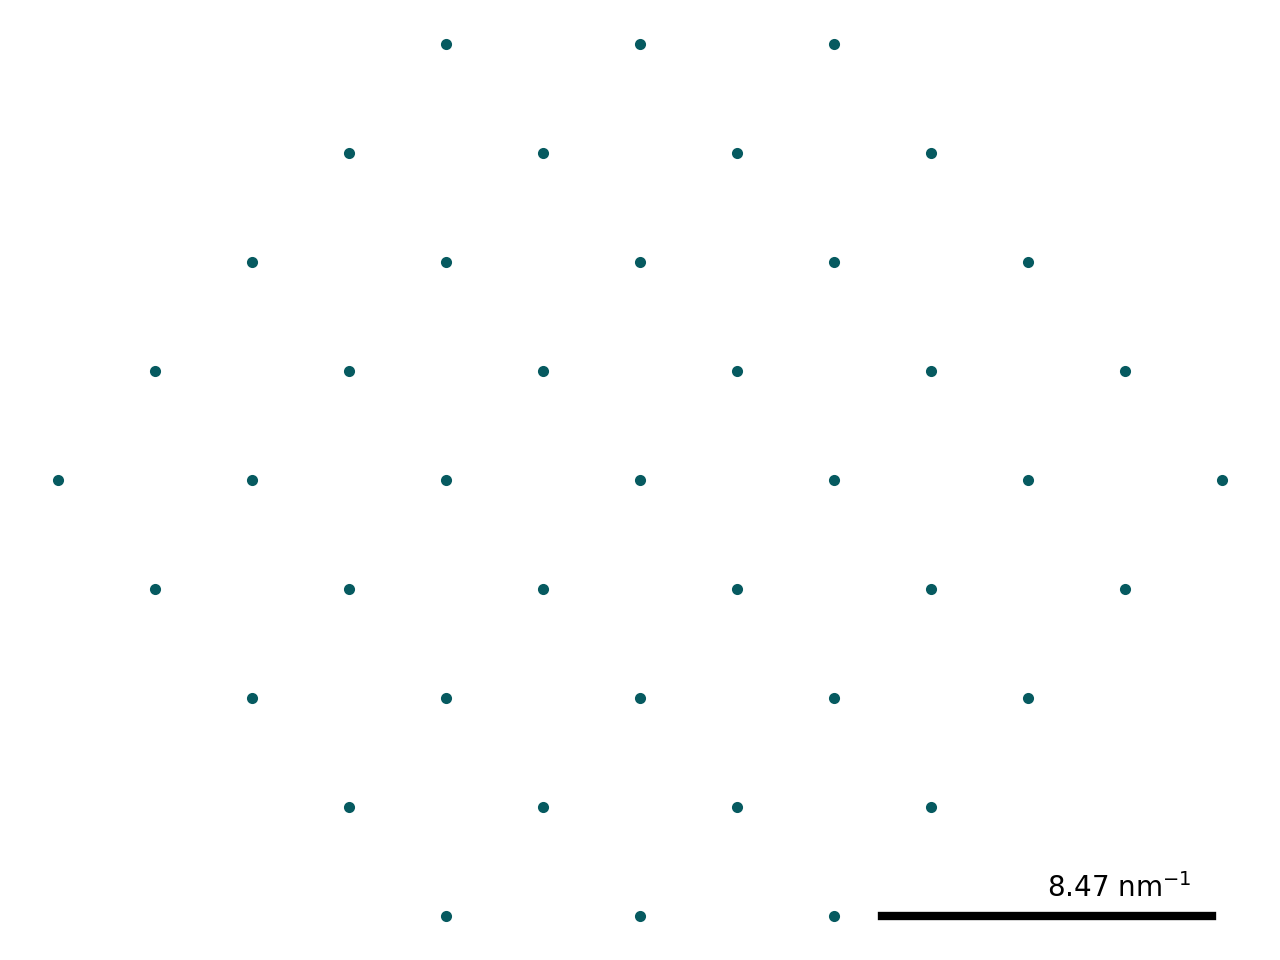
\includegraphics[scale=0.4]{../Graphics/inicial.png}
    \caption{Configuración de los átomos de Plata}
    \label{fig:inicial}
\end{figure}
La Configuración de posiciones de los átomos de plata en nuestro material cristalino son los mostrados en la figura \ref{fig:inicial}.\\
Para poder identificar que distancias interatomicas son importante para el estudio se propusieron las siguientes condiciones:\\
Dado un punto de referencia llamado centro u órigen y dos puntos i,j tal que $i\neq j$  se tiene que cumplir que:
\begin{enumerate}
    \item La distancia entre el centro e i, tiene que ser la misma entre el centro y j.
    \item La pendiente de los putnos del centro e i y el centro y j tiene que ser iguales.
\end{enumerate}
\section{Resultados}
Para el caso mostrado, en la figura \ref{fig:inicial}, se propuso como átomo de origen el que se encuentra en la parte central, por lo que
desarrollando un algoritmo lea las posiciones de todos los átomos e imprima las distancias interatomicas en una gráfica para observar sus relaciones,
la figura generada es la figura \ref{fig:distancias}.
\begin{figure}[H]
    \centering
    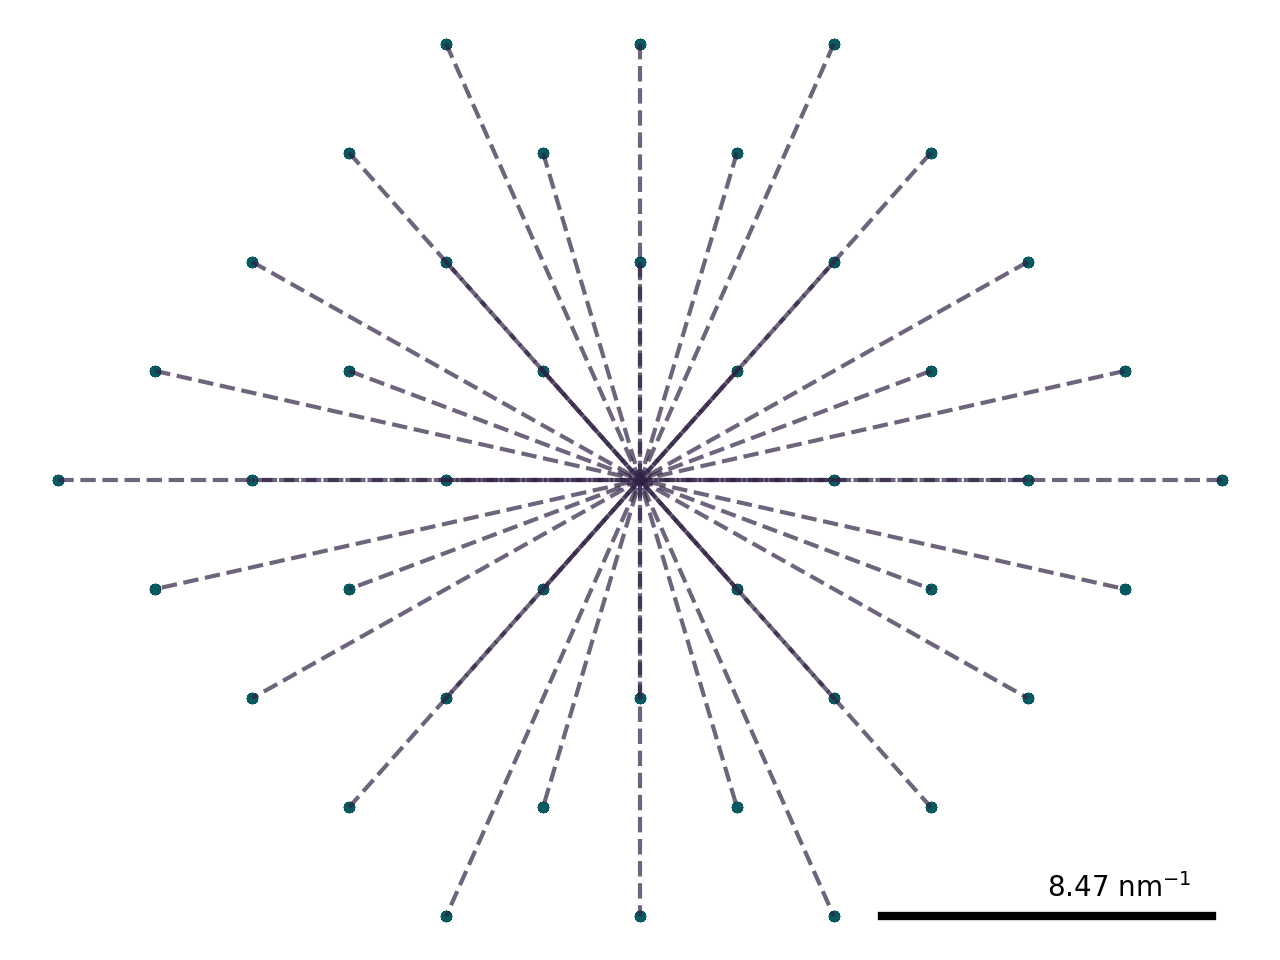
\includegraphics[scale=0.4]{../Graphics/distancia.png}
    \caption{Distancias interatomicas calculadas usando las condiciones entre tres puntos.}
    \label{fig:distancias}
\end{figure}
A la par el algoritmo calcula las distancias interatomicas que cumplan las condiciones, con ello realiza una relación con los parámetros mostrados en la tabla \ref{tabla:parametros},
llegando así a encontrar las familias de los indices de Miller para todos los átomos de plata, estos indices estan mostrados en la 
figura \ref{fig:indicesmiller}. \\
\begin{figure}[H]
    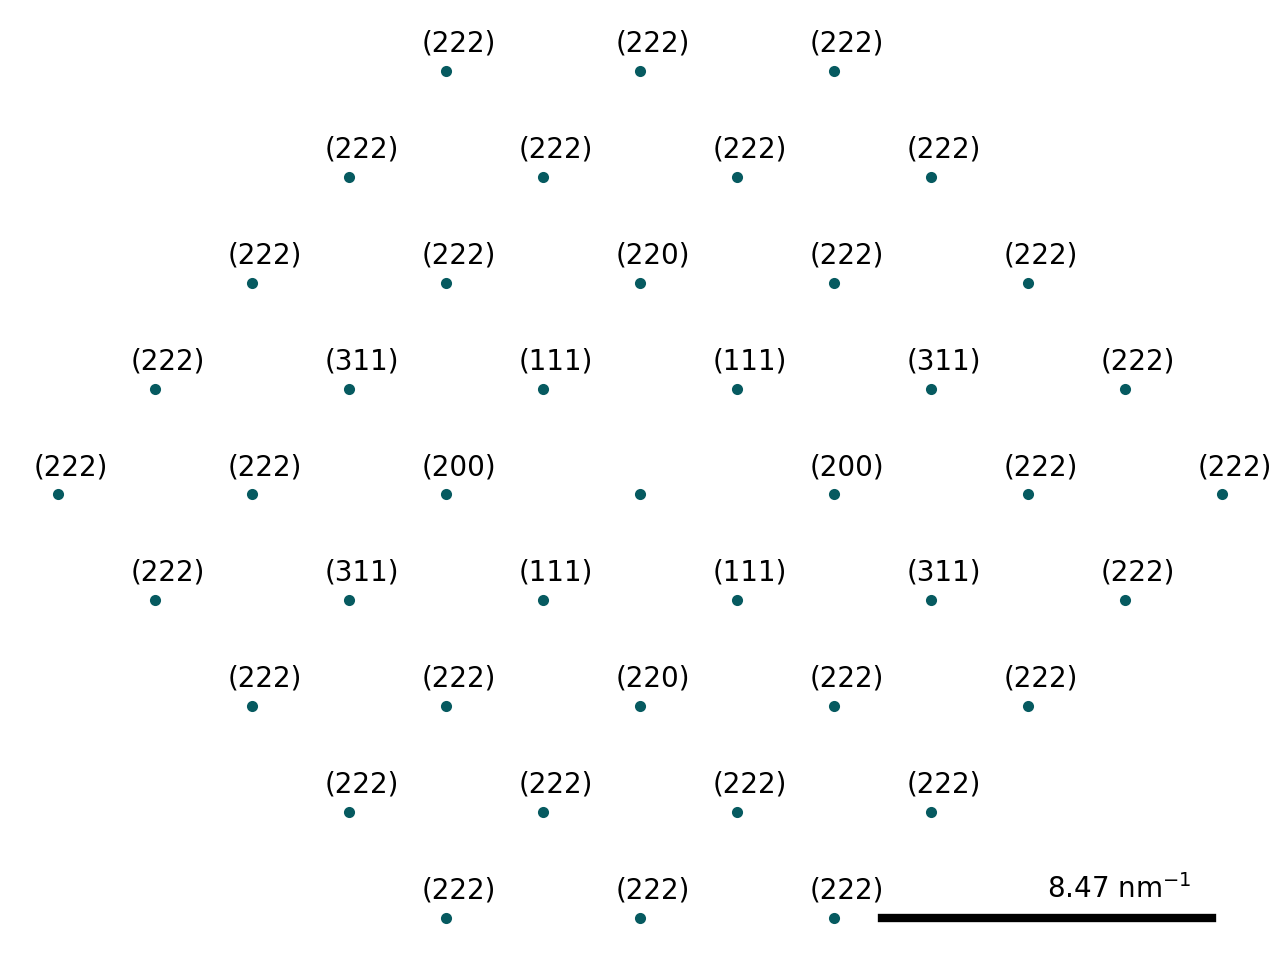
\includegraphics[scale=0.45]{../Graphics/indices.png}
    \caption{Familia de indices de Miller asignados a partir de los datos de la tabla \ref{tabla:parametros} usando el código \ref{cod:distancias}}
    \label{fig:indicesmiller}
\end{figure}
A partir de la familia (111) se calcularon los indices particulares para cada posición, esto haciendo uso de propiedades vectoriles, para 
así obtener los indices mostrados en la figura \ref{fig:lattice}.
\begin{figure}[H]
    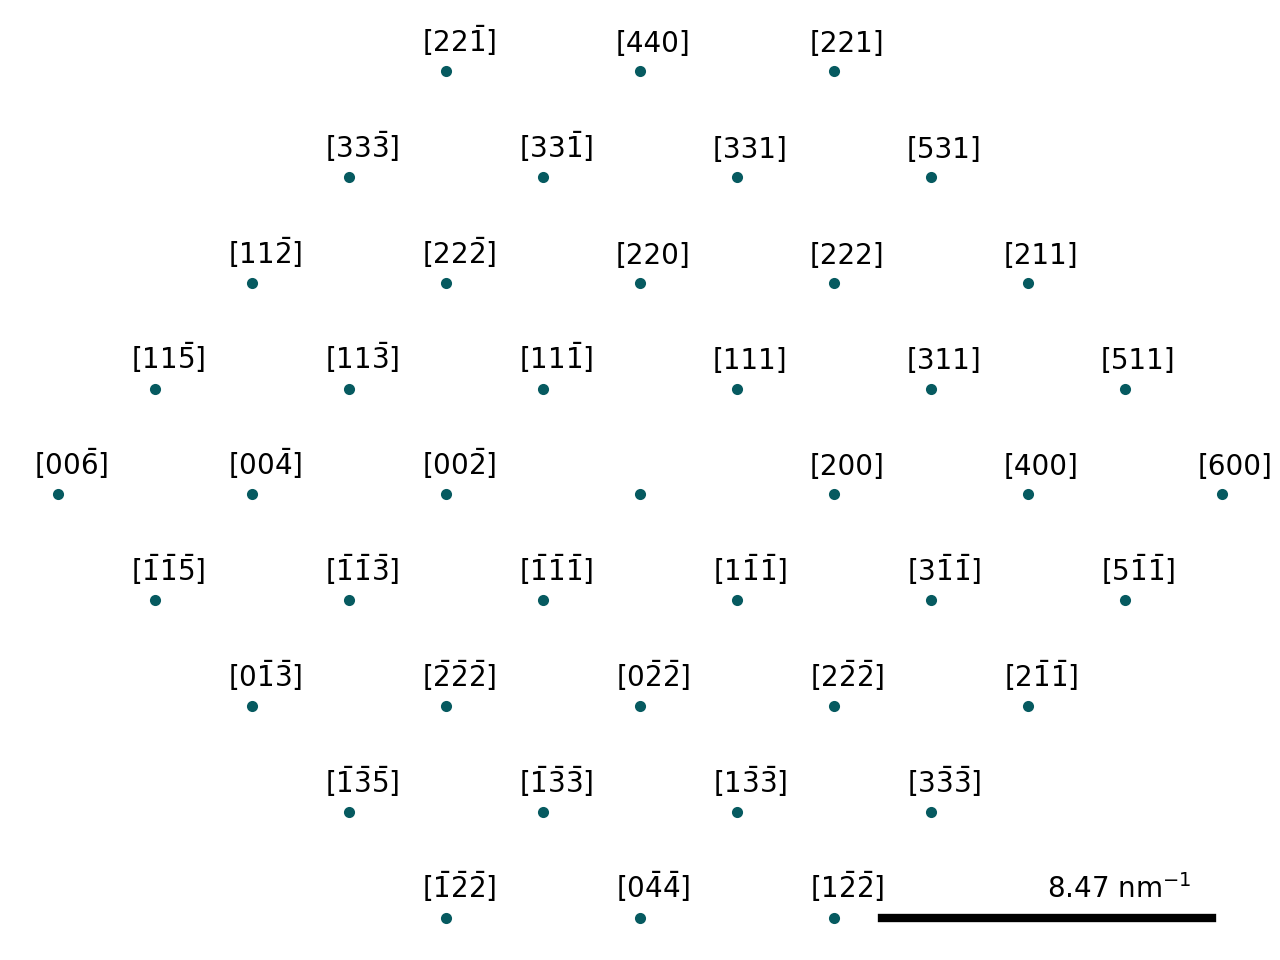
\includegraphics[scale=0.45]{../Graphics/lattice.png}
    \caption{Indices de Miller asignados a partir de la suma vectorial con los indices de la familia (111) como valores iniciales.}
    \label{fig:lattice}
    \end{figure}
\section{Conclusiones}
La implementación de las herramientas computacionales junto con las tecnologicas pueden dar a conocer a mayor detalle los objetos de estudio, 
ya que el calculo y obtención de datos se realiza de una forma eficaz para realizar los procedimientos necesarios, en este caso que aunque solo le hayamos
introducido una condición de simetria con respecto a las distancias, el algoritmos regreso una simetria en base a los indices de Miller dentro del sistema de átomos
propuesto.
\section{Código}
\begin{enumerate}
    \item \href{https://github.com/giovannilopez9808/Notas_Agosto_2020/blob/master/AMC/Tarea2/distancia.py}{Distancia.py\label{cod:distancias}}\\
    Este código realiza las figuras \ref{fig:inicial}, \ref{fig:distancias}, \ref{fig:indicesmiller} y \ref{fig:lattice} a partir de la posición de los átomos y la información de la tabla \ref{tabla:parametros}
\end{enumerate}
\bibliographystyle{plain}
\nocite{*}
\bibliography{Main}
\end{document}